\section{Matter}

\begin{multicols}{2}


\section*{Concept of Matter}


\subsection{Air is Matter}

\begin{center}
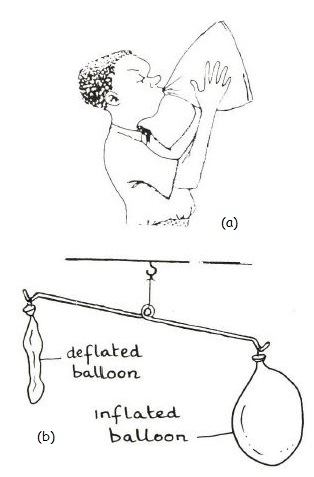
\includegraphics[width=0.4\textwidth]{./img/source/air-matter.jpg}
\end{center}

\begin{description*}
%\item[Subtopic:]{}
%\item[Materials:]{Balloons/plastic bags, wire}
%\item[Setup:]{}
\item[Procedure:]{Blow a bag or balloon up with air (a). Hang a deflated bag and an inflated bag on either side of a simple wire balance.}
%\item[Hazards:]{}
%\item[Questions:]{}
\item[Observations:]{Air in the bag occupies space. The air has mass as indicated by the balance.}
%\item[Theory:]{}
%\item[Applications:]{}
%\item[Notes:]{}
\end{description*}

\subsection{Liquid is Matter}

\begin{center}
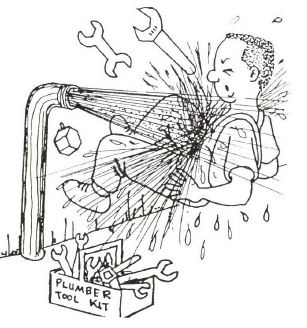
\includegraphics[width=0.4\textwidth]{./img/source/liquid-matter.jpg}
\end{center}

\begin{description*}
%\item[Subtopic:]{}
%\item[Materials:]{}
%\item[Setup:]{}
%\item[Procedure:]{}
%\item[Hazards:]{}
%\item[Questions:]{}
%\item[Observations:]{}
\item[Theory:]{Liquids contain mass, occupy space and can provide a great force under pressure. Don't be like the plumber in the picture!}
%\item[Applications:]{}
%\item[Notes:]{}
\end{description*}

%==================================================================================================%

\section*{States of Matter}
All matter is made up of particles. These particles are in constant motion which increases with their temperature. Depending on temperature, matter may exist in three states: \emph{solid}, \emph{liquid} or \emph{gas}.
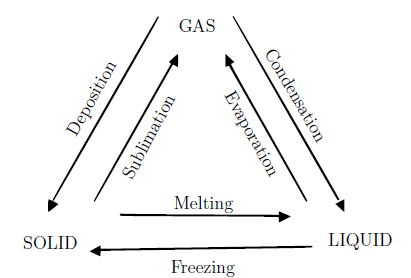
\includegraphics[width=0.4\textwidth]{./img/changes-of-state.png}

\subsection{Students as Matter}

\begin{center}
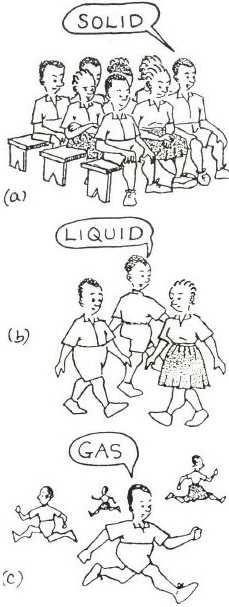
\includegraphics[width=0.4\textwidth]{./img/source/states-matter-students.jpg}
%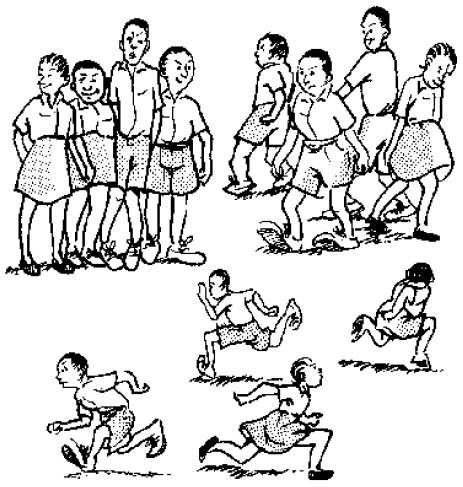
\includegraphics[width=0.4\textwidth]{./img/vso/states-matter.png}
\end{center}

\begin{description*}
%\item[Subtopic:]{}
%\item[Materials:]{}
%\item[Setup:]{}
\item[Procedure:]{Use students to demonstrate the concept of states of matter.}
%\item[Hazards:]{}
%\item[Questions:]{}
%\item[Observations:]{}
\item[Theory:]{When students or objects are close together, they represent particles in the \emph{solid} state. As they move apart and past each other they represent particles in the \emph{liquid} state. Fast and randomly moving pupils or objects represent particles in the \emph{gaseous} state.}
%\item[Applications:]{}
%\item[Notes:]{}
\end{description*}

\subsection{Arranging States of Matter}

\begin{center}
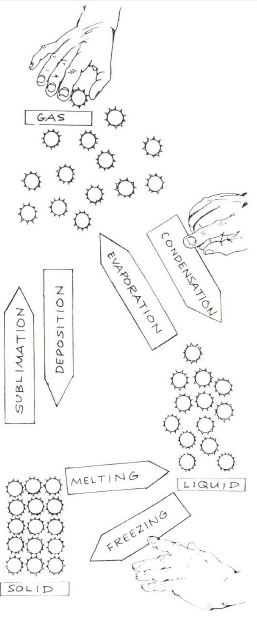
\includegraphics[width=0.4\textwidth]{./img/source/state-arranging.jpg}
\end{center}

\begin{description*}
%\item[Subtopic:]{}
\item[Materials:]{Bottle caps, paper}
%\item[Setup:]{}
\item[Procedure:]{Have students arrange bottle caps to represent the different states of matter, using labels from paper or cardboard.}
%\item[Hazards:]{}
%\item[Questions:]{}
%\item[Observations:]{}
\item[Theory:]{The spacing of the bottle caps represents the distance between particles in each state. Particles have large spaces between them in gases, less space in liquids, and are very condensed in solids.}
%\item[Applications:]{}
%\item[Notes:]{}
\end{description*}

\subsection{A Model of Motion}

\begin{center}
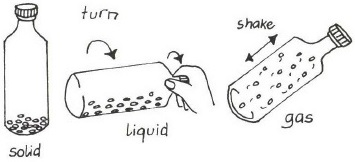
\includegraphics[width=0.49\textwidth]{./img/vso/motion-model.jpg}
\end{center}

\begin{description*}
%\item[Subtopic:]{}
%\item[Materials:]{}
%\item[Setup:]{}
\item[Procedure:]{Put some dry beans, rice or stones in a clear bottle. Hold the bottle still, then turn it, then shake it vigorously.}
%\item[Hazards:]{}
\item[Questions:]{Which activity corresponds to which state of matter?}
%\item[Observations:]{}
\item[Theory:]{The movement of particles in solids is small and hence they are in fixed order. In liquids the particles move past each other and have lost the stiff order. In gases they move very fast and randomly, losing all order.}
%\item[Applications:]{}
%\item[Notes:]{}
\end{description*}

\subsection{Physical and Chemical Changes}

\begin{center}
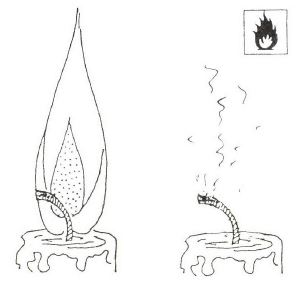
\includegraphics[width=0.4\textwidth]{./img/source/physical-change.jpg}
\end{center}

\begin{description*}
%\item[Subtopic:]{}
\item[Materials:]{Candle, paper, sugar, bottle caps}
%\item[Setup:]{}
\item[Procedure:]{Light a candle and let it drip into a bottle cap. Then light the paper and catch the remains in another cap. Finally place a small amount of sugar in a cap and heat it over the flame.}
%\item[Hazards:]{}
%\item[Questions:]{}
\item[Observations:]{The candle wax melts into a liquid, then upon cooling reforms into a solid. The paper burns up and leaves ash. The sugar turns brown upon heating, leaving a brownish black solid upon cooling.}
\item[Theory:]{The candle wax undergoes a physical change that only affects its physical properties. After heating, we can get the original wax back again by cooling. The paper and sugar undergo chemical changes since the change is not reversible.}
%\item[Applications:]{}
%\item[Notes:]{}
\end{description*}

%==================================================================================================%

\section*{Elements and Symbols}


\subsection{Element Memory Game} % PIC!!!

%\begin{center}
%\includegraphics[width=0.4\textwidth]{./img/.jpg}
%\end{center}

\begin{description*}
%\item[Subtopic:]{}
\item[Materials:]{Manila paper/card/paper}
\item[Setup:]{Cut out 2 sets of identical small squares of card or paper. On the first set write the names of some elements and on the second set write their corresponding symbols. Make about 10-15 pairs. }
\item[Procedure:]{Mix the cards together and spread them out on a table face down. Students take turns flipping over 2 cards at a time. If the element and symbol match, they get to keep the cards. If not, they must turn them back over. The player with the most pairs of cards at the end wins!}
%\item[Hazards:]{}
%\item[Questions:]{}
%\item[Observations:]{}
%\item[Theory:]{}
%\item[Applications:]{}
%\item[Notes:]{}
\end{description*}

%==================================================================================================%

\section*{Compounds and Mixtures}


\subsection{Introducing Mixtures}

\begin{center}
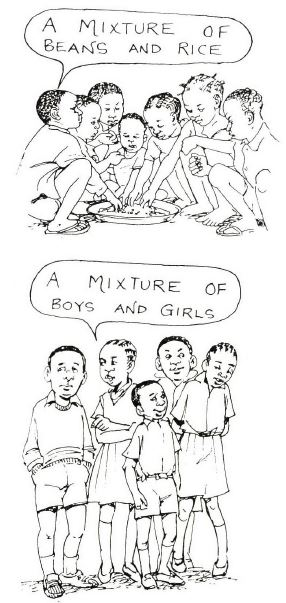
\includegraphics[width=0.4\textwidth]{./img/source/intro-mixtures.jpg}
\end{center}

\begin{description*}
%\item[Subtopic:]{}
%\item[Materials:]{}
%\item[Setup:]{}
\item[Procedure:]{Why not introduce mixrures with a
game? Students will like a more concrete
introduction. Try it!}
%\item[Hazards:]{}
%\item[Questions:]{}
%\item[Observations:]{}
%\item[Theory:]{}
%\item[Applications:]{}
%\item[Notes:]{}
\end{description*}

\subsection{Student Compounds}

\begin{center}
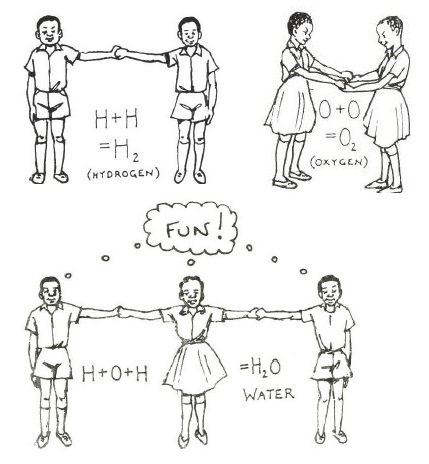
\includegraphics[width=0.45\textwidth]{./img/source/student-compounds.jpg}
\end{center}

\begin{description*}
%\item[Subtopic:]{}
%\item[Materials:]{}
%\item[Setup:]{}
\item[Procedure:]{To show that elements combine in constant
proportions, ask the students to play a game of
forming molecules like those of water, ammonia,
methane, ethane, carbon dioxide etc. See the
figures.}
%\item[Hazards:]{}
%\item[Questions:]{}
%\item[Observations:]{}
%\item[Theory:]{}
%\item[Applications:]{}
%\item[Notes:]{}
\end{description*}

\subsection{Mixtures and Compounds}

\begin{center}
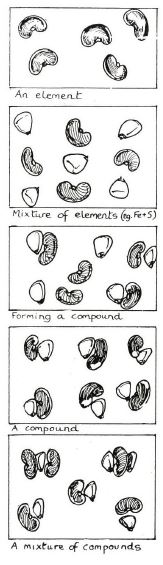
\includegraphics[width=0.35\textwidth]{./img/source/mixtures-compounds.jpg}
\end{center}

\begin{description*}
%\item[Subtopic:]{}
\item[Materials:]{Beans, seeds, corn kernels, etc.}
%\item[Setup:]{}
\item[Procedure:]{Use the items to represent various elements, mixtures and compounds as shown.}
%\item[Hazards:]{}
%\item[Questions:]{}
%\item[Observations:]{}
\item[Theory:]{In homogeneous mixtures, the particles are
uniformly mixed and it is impossible to see the
different ingredients even by using a light
microscope. For example, solutions and the
mixture of gases in air are homogeneous
mixtures.

In heterogeneous mixtures, the particles are
also uniformly mixed. But the individual
components can be seen either by eye or by
using a magnifying glass or microscope.}
%\item[Applications:]{}
%\item[Notes:]{}
\end{description*}

\subsection{Heterogeneous Mixtures}

\begin{center}
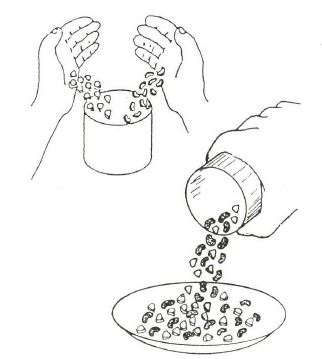
\includegraphics[width=0.4\textwidth]{./img/source/heterogeneous.jpg}
\end{center}

\begin{description*}
%\item[Subtopic:]{}
\item[Materials:]{Bean seeds, maize grains, salt, sand, sugar}
%\item[Setup:]{}
\item[Procedure:]{(a) Take a handful of maize grains and
another handful of bean seeds. Each handful is
like a pure substance having only one kind of
particle. Now mix the maize grains and the
beans in a container. 
Repeat with sand and salt or sand and sugar.}
%\item[Hazards:]{}
%\item[Questions:]{}
%\item[Observations:]{}
\item[Theory:]{This is like a heterogeneous
mixture since different particles can be seen.}
\item[Applications:]{Common everyday examples of
heterogenous mixtures are turbid water and
porridge. Preparing concrete is another example which can be observed in daily life.}
%\item[Notes:]{}
\end{description*}

\subsection{Homogeneous Mixtures}

\begin{center}
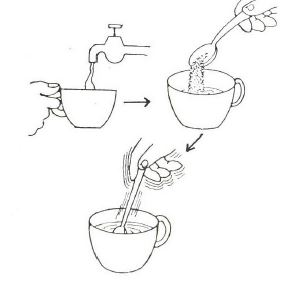
\includegraphics[width=0.4\textwidth]{./img/source/homogeneous.jpg}
\end{center}

\begin{description*}
%\item[Subtopic:]{}
\item[Materials:]{Salt, water, spoon, bottle}
%\item[Setup:]{}
\item[Procedure:]{Dissolve some table salt or sugar in drinking
water to demonstrate a solution as a
homogeneous mixture. Ask the pupils to taste
the solution to prove that the chemical properties
of the solute have not changed.}
\item[Hazards:]{Ensure that clean water, cups and spoons
are used.}
%\item[Questions:]{}
%\item[Observations:]{}
%\item[Theory:]{}
%\item[Applications:]{}
%\item[Notes:]{}
\end{description*}

\subsection{Separating Iron and Sulphur} % VSO 63

\begin{center}
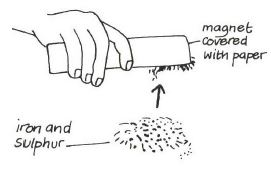
\includegraphics[width=0.4\textwidth]{./img/vso/iron-sulphur.jpg}
\end{center}

\begin{description*}
%\item[Subtopic:]{}
\item[Materials:]{Steel wool, sulphur powder, magnet, paper}
\item[Setup:]{Prepare a mixture of iron filings and sulphur powder.}
\item[Procedure:]{Cover the magnet with paper.
The magnet will attract only the
iron, leaving sulphur behind.}
%\item[Hazards:]{}
%\item[Questions:]{}
%\item[Observations:]{}
\item[Theory:]{The magnetic properties of the iron filings allow the magnet to separate the mixture by attracting the iron.}
%\item[Applications:]{}
%\item[Notes:]{}
\end{description*}

\subsection{Types of Solutions} % PIC!!! Shika 296

%\begin{center}
%\includegraphics[width=0.4\textwidth]{./img/.jpg}
%\end{center}

\begin{description*}
%\item[Subtopic:]{}
\item[Materials:]{3 cups, water, salt, spoon}
%\item[Setup:]{}
\item[Procedure:]{Fill 3 cups with water. In the first add a bit of salt. In the second, add salt unitl it no longer dissolves. In the third, add salt until a small mound forms on the bottom. Stir each solution and taste a small amount.}
%\item[Hazards:]{}
%\item[Questions:]{}
\item[Observations:]{Cup 1 tastes slightly salty, while cups 2 and 3 taste the same - very salty.}
\item[Theory:]{Cup 1 contains an \emph{unsaturated} solution, i.e. it can still dissolve more salt. Cup 2 has a \emph{saturated} solution - it can dissolve no more salt. Cup 3 has a \emph{supersaturated} solution - it holds more undissolved salt at the bottom.}
%\item[Applications:]{}
%\item[Notes:]{}
\end{description*}

%\subsection{Solutions, Suspensions and Emulsions} % LASM 48
%
%%\begin{center}
%%\includegraphics[width=0.4\textwidth]{./img/.jpg}
%%\end{center}
%
%\begin{description*}
%%\item[Subtopic:]{}
%\item[Materials:]{}
%\item[Setup:]{}
%\item[Procedure:]{}
%\item[Hazards:]{}
%\item[Questions:]{}
%\item[Observations:]{}
%\item[Theory:]{}
%\item[Applications:]{}
%\item[Notes:]{}
%\end{description*}

\subsection{Suspensions}

\begin{center}
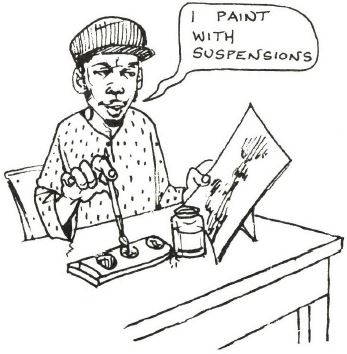
\includegraphics[width=0.4\textwidth]{./img/source/suspensions.jpg}
\end{center}

\begin{description*}
%\item[Subtopic:]{}
%\item[Materials:]{}
%\item[Setup:]{}
%\item[Procedure:]{}
%\item[Hazards:]{}
%\item[Questions:]{}
%\item[Observations:]{}
\item[Theory:]{A suspension is a mixture of a solid and a
liquid. Suspensions can be made from solids
like sand, soil, ash, sawdust etc. with a liquid
like water. }
\item[Applications:]{Let the students find more examples
from their daily life (e.g. toothpaste and
porridge).}
%\item[Notes:]{}
\end{description*}

\subsection{Emulsions} % Source 93, Shika 288

\begin{center}
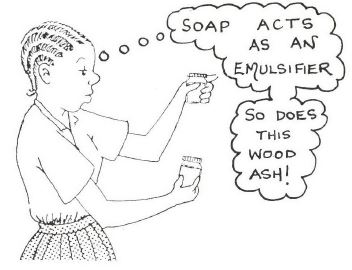
\includegraphics[width=0.4\textwidth]{./img/source/emulsions.jpg}
\end{center}

\begin{description*}
%\item[Subtopic:]{}
\item[Materials:]{Kerosene/oil, water, bottle, soap}
%\item[Setup:]{}
%\item[Procedure:]{}
%\item[Hazards:]{}
%\item[Questions:]{}
%\item[Observations:]{}
\item[Theory:]{Emulsions are made from two immiscible
liquids like kerosene or oil in water. Shake and
let it stand for some time to demonstrate an
unstable emulsion. If soap is added to the water
it acts as an emulsifier and stabilizes the
emulsion. Wood ash also acts in this way. }
\item[Applications:]{Let the students find more examples in
daily life (e.g. milk).}
%\item[Notes:]{}
\end{description*}

\subsection{Miscible and Immiscible Liquids} % Source 93, Shika 287

\begin{center}
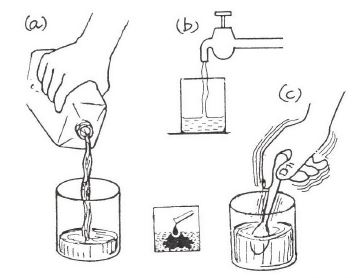
\includegraphics[width=0.4\textwidth]{./img/source/miscible-immiscible.jpg}
\end{center}

\begin{description*}
%\item[Subtopic:]{}
\item[Materials:]{Water, kerosene, alcohol, bottles}
%\item[Setup:]{}
\item[Procedure:]{Mix equal amounts of water separately with
kerosene and alcohol in two different containers.}
\item[Hazards:]{Kerosene is water polluting! Do not pour it
into the sink. Keep it in a labeled container for
further experiments.}
%\item[Questions:]{}
%\item[Observations:]{}
\item[Theory:]{The water and kerosene combine to make an immiscible liquid, whereas the water and alcohol form a miscible liquid.}
%\item[Applications:]{}
%\item[Notes:]{}
\end{description*}

\subsection{Lava Lamp} % PIC!!! Shika 286

%\begin{center}
%\includegraphics[width=0.4\textwidth]{./img/.jpg}
%\end{center}

\begin{description*}
%\item[Subtopic:]{}
\item[Materials:]{Bottle, water, food coloring, oil, effervescing
antacid tablets, 
ashlight,}
%\item[Setup:]{}
\item[Procedure:]{Fill the bottom 10 cm of a water bottle with water. Add
a few drops of food coloring. Fill rest of the bottle with oil. Drop in
an effervescing antacid tablet. Cap and put a 
flashlight underneath the
bottle. }
%\item[Hazards:]{}
%\item[Questions:]{}
\item[Observations:]{Observe the colors and the movement of the liquids.}
\item[Theory:]{Oil is a compound that is hydrophobic (it repels
water). Oil is a long non-polar hydrocarbon, while water
is a small polar compound. This means that the water cannot mix with
the oil layer. This is why there are two layers on mixing oil and water.
Adding the effervescing antacid tablets dissolve and release carbon dioxide
in the water layer. The carbon dioxide dissolves in the water and forms
small bubbles of carbon dioxide. These bubbles trap small amounts of
food coloring. These bubbles rise since they have a much lower density
than water. When the bubble reaches the surface, the carbon dioxide
escapes and the colored water bubble falls down through the oil layer.}
%\item[Applications:]{}
%\item[Notes:]{}
\end{description*}

\subsection{Moving Colours} % PIC!!! Shika 286

%\begin{center}
%\includegraphics[width=0.4\textwidth]{./img/.jpg}
%\end{center}

\begin{description*}
%\item[Subtopic:]{}
\item[Materials:]{Milk, various food colouring, powdered soap, cotton ball or swab, shallow dish or plate}
%\item[Setup:]{}
\item[Procedure:]{Pour in just enough milk to cover the plate or the bowl. Place a few drops of
food colouring around the plate of milk. Soak
the cotton swab in some soapy water and touch it to the center of the
milk plate. }
%\item[Hazards:]{}
%\item[Questions:]{}
\item[Observations:]{The colours will start to move and
swirl towards the center.}
\item[Theory:]{Milk is made up of fats and different proteins (non-polar molecules). The water solution in the food colour and the non polar milk barely mix. Soap
is a compound that is both polar on one end and non polar on the other
end. The milk and the soap intermingle forming micelles. In addition,
the surface tension of the water in the milk breaks, allowing
food colouring to move around in the milk. }
%\item[Applications:]{}
%\item[Notes:]{}
\end{description*}

%==================================================================================================%

\section*{Separating Mixtures}


\subsection{Decantation}

\begin{center}
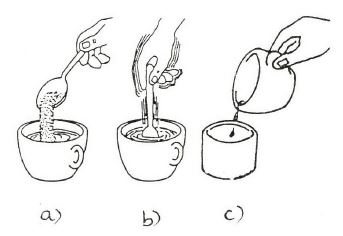
\includegraphics[width=0.4\textwidth]{./img/source/decantation.jpg}
\end{center}

\begin{description*}
%\item[Subtopic:]{}
\item[Materials:]{Cup, water, sand}
%\item[Setup:]{}
\item[Procedure:]{This procedure is based on the different
density of particles.
Shake some sand with water, let it stand for
some time and decant the water.}
%\item[Hazards:]{}
%\item[Questions:]{}
%\item[Observations:]{}
%\item[Theory:]{}
\item[Applications:]{Maize seeds are usually washed before milling.
After washing the maize seeds are separated
from the water by decantation.}
%\item[Notes:]{}
\end{description*}

\subsection{Evaporation}

\begin{center}
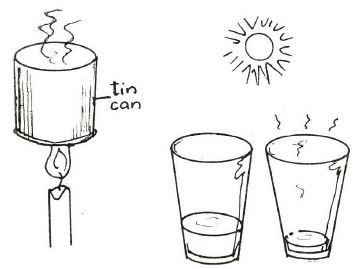
\includegraphics[width=0.4\textwidth]{./img/source/evaporation.jpg}
\end{center}

\begin{description*}
%\item[Subtopic:]{}
\item[Materials:]{Container, salt, water}
%\item[Setup:]{}
\item[Procedure:]{This procedure is based on different
boiling points.
(a) Dissolve some common salt in water and
heat to dryness.
(b) Better crystals can be obtained by evaporating
most of the water. The remaining water can be
evaporated slowly in the sun.}
%\item[Hazards:]{}
%\item[Questions:]{}
%\item[Observations:]{}
%\item[Theory:]{}
%\item[Applications:]{}
%\item[Notes:]{}
\end{description*}

\subsection{Distillation}

\begin{center}
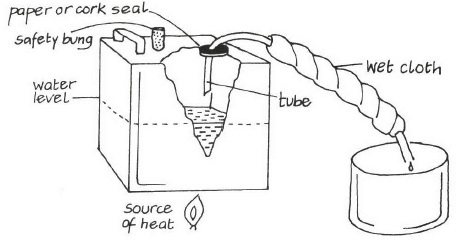
\includegraphics[width=0.49\textwidth]{./img/vso/distillation.jpg}
\end{center}

\begin{description*}
%\item[Subtopic:]{}
\item[Materials:]{Metal can, cork/rubber stopper, plastic tubing, wet cloth, container, \nameref{sec:heatsources}}
%\item[Setup:]{}
\item[Procedure:]{Fill a container half way with water. Cut a hole in the top and fix a rubber stopper with a plastic tube through the center. Wrap a wet cloth around the tube and feed it into a can. Add a safety bung using rubber or cork to prevent against very high pressures within the container and place the container over the heat source.}
\item[Hazards:]{Make sure the safety bung is not too tight and that the container always has water inside.}
%\item[Questions:]{}
%\item[Observations:]{}
\item[Theory:]{Heating the can produces steam which is then cooled by the wet cloth. Steam condenses to produce water.}
\item[Applications:]{This method can be used to purify water.}
%\item[Notes:]{}
\end{description*}

\subsection{Distillation of a Solution}

\begin{center}
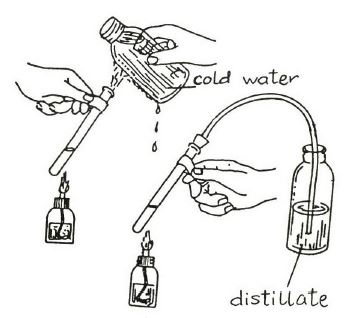
\includegraphics[width=0.4\textwidth]{./img/distillation-solution.jpg}
\end{center}

\begin{description*}
%\item[Subtopic:]{}
\item[Materials:]{Candle, bottles, cold water, ash extract, tube}
%\item[Setup:]{}
\item[Procedure:]{Take the ash extract obtained by filtration and distill it as shown. The
ash extract is separated into a liquid (distillate)
and a solid residue.}
\item[Hazards:]{Take care due to the small diameter of the
connection tubes.}
%\item[Questions:]{}
%\item[Observations:]{}
\item[Theory:]{The solids have a much higher boiling point
than the water.}
%\item[Applications:]{}
%\item[Notes:]{}
\end{description*}

\subsection{Separating Immiscible Liquids} % VSO 63

\begin{center}
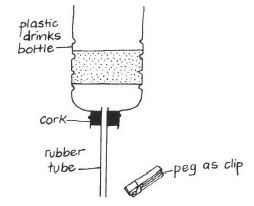
\includegraphics[width=0.4\textwidth]{./img/vso/sep-immiscible.jpg}
\end{center}

\begin{description*}
%\item[Subtopic:]{}
\item[Materials:]{Kerosene, water, bottle, cork, rubber tube, clothespin}
%\item[Setup:]{}
\item[Procedure:]{Combine 2 liquids together that do not mix well, e.g. groundnut oil and water; palm oil
and water; petrol/diesel and
water; castor oil and water. Palm
oil is particularly effective because
it is brightly coloured.}
%\item[Hazards:]{}
%\item[Questions:]{}
%\item[Observations:]{}
\item[Theory:]{When 2 liquids will not mix with
each other they are said to be
immiscible. One liquid will sink
below the other and can be
drawn off as shown.}
%\item[Applications:]{}
%\item[Notes:]{}
\end{description*}

\subsection{Filtration}

\begin{center}
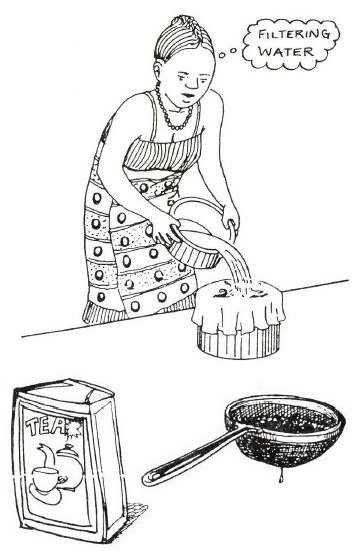
\includegraphics[width=0.4\textwidth]{./img/source/filtering.jpg}
\end{center}

\begin{description*}
%\item[Subtopic:]{}
%\item[Materials:]{}
%\item[Setup:]{}
%\item[Procedure:]{}
%\item[Hazards:]{}
%\item[Questions:]{}
%\item[Observations:]{}
\item[Theory:]{Filtering is based on the same principle as
sieving. It is a frequently used process in daily
life. The students can explain different filtering
processes they know.}
%\item[Applications:]{}
%\item[Notes:]{}
\end{description*}

\subsection{Chromatography} % Source 97, LASM 56, Shika 247

\begin{center}
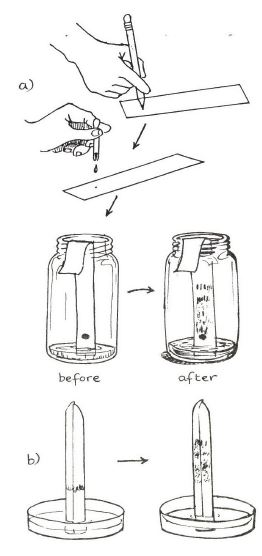
\includegraphics[width=0.4\textwidth]{./img/source/chromatography.jpg} 
\end{center}

\begin{description*}
%\item[Subtopic:]{}
\item[Materials:]{Pen/marker, newspaper, water, chalk, ink}
%\item[Setup:]{}
\item[Procedure:]{(a) Make a line with ink or a black felt pen (containing water soluble
colour) on a strip made from filter paper or the white rim of a newspaper. Hang the strip into
water, so that the spot is above the water level.

(b) Stand a piece of chalk in ink. The chalk must
stand upright.}
%\item[Hazards:]{}
%\item[Questions:]{}
%\item[Observations:]{}
\item[Theory:]{This procedure is based on the differeni
capillary rise of soluble substances in a porous
support. Many colours are mixtures. The different
colours rise at different speeds and thus separate.}
%\item[Applications:]{}
%\item[Notes:]{}
\end{description*}

%==================================================================================================%


\end{multicols}

\pagebreak